\section{Swing Prediction Model}

\subsection{Model Introduction}~{}

To predict the swings, we need to find potential factors that may affect future momentum.
In problem 1, we established a standard to judge the player's performance;
in problem 2, we found the player's performance, ``momentum'', has a one order of autocorrelation,
which indicates that some factors of the momentum have impact on the future momentum.

To find what and how factors affect the future momentum, we can take advantage 
of Machine Learning. In this section, we will primarily focus on establishing a 
supervised learning classification model using the Gated Recurrent Unit (GRU) network to 
predict momentum swings. We will break down the problems into three parts:

\begin{itemize}
    \item definition of the swing of the play
    \item data (potential factors) and label used to train GRU
    \item Utilizing Gated Recurrent Unit
\end{itemize}

\subsubsection{Definition of ``Swings of the Play''}~{}

We first give the definition of the swings of the play.
Based on our previous definition of ``momentum,'' the significant changes of the game 
largely depend on the ``momentum'' of the two players. Therefore, we choose ``momentum'' to represent 
the swings of the play. The specific definition is as follows:\\

We use $\Delta f(t)$ to represent the difference in ``momentum'' between the two players., 
so it can be easily seen that if $\Delta f(t)$ and $\Delta f(t+1)$
have different signs, it indicates a ``swing'' in the game's momentum. 
In this way, we can define four states of ``momentum'' at time $t$:

$$states=\begin{cases}
    state1, &\text{if } \Delta f(t)>0 \text{ and } \Delta f(t+1)>0, \text{ which means stay positive}\\
    state2, &\text{if } \Delta f(t)<0 \text{ and } \Delta f(t+1)>0, \text{ which means rise from negative to positive}\\
    state3, &\text{if } \Delta f(t)<0 \text{ and } \Delta f(t+1)<0, \text{ which means stay negative}\\
    state4, &\text{if } \Delta f(t)>0 \text{ and } \Delta f(t+1)<0, \text{ which means decrease from positive to negative}
\end{cases}$$
Obviously, if state 2 or state 4 appears, we can determine that a swing has occurred. 

To visualize the swing, we choose four shapes of lines to represent the four states of swings at time $t$:

\begin{figure}[H]
    \centering
        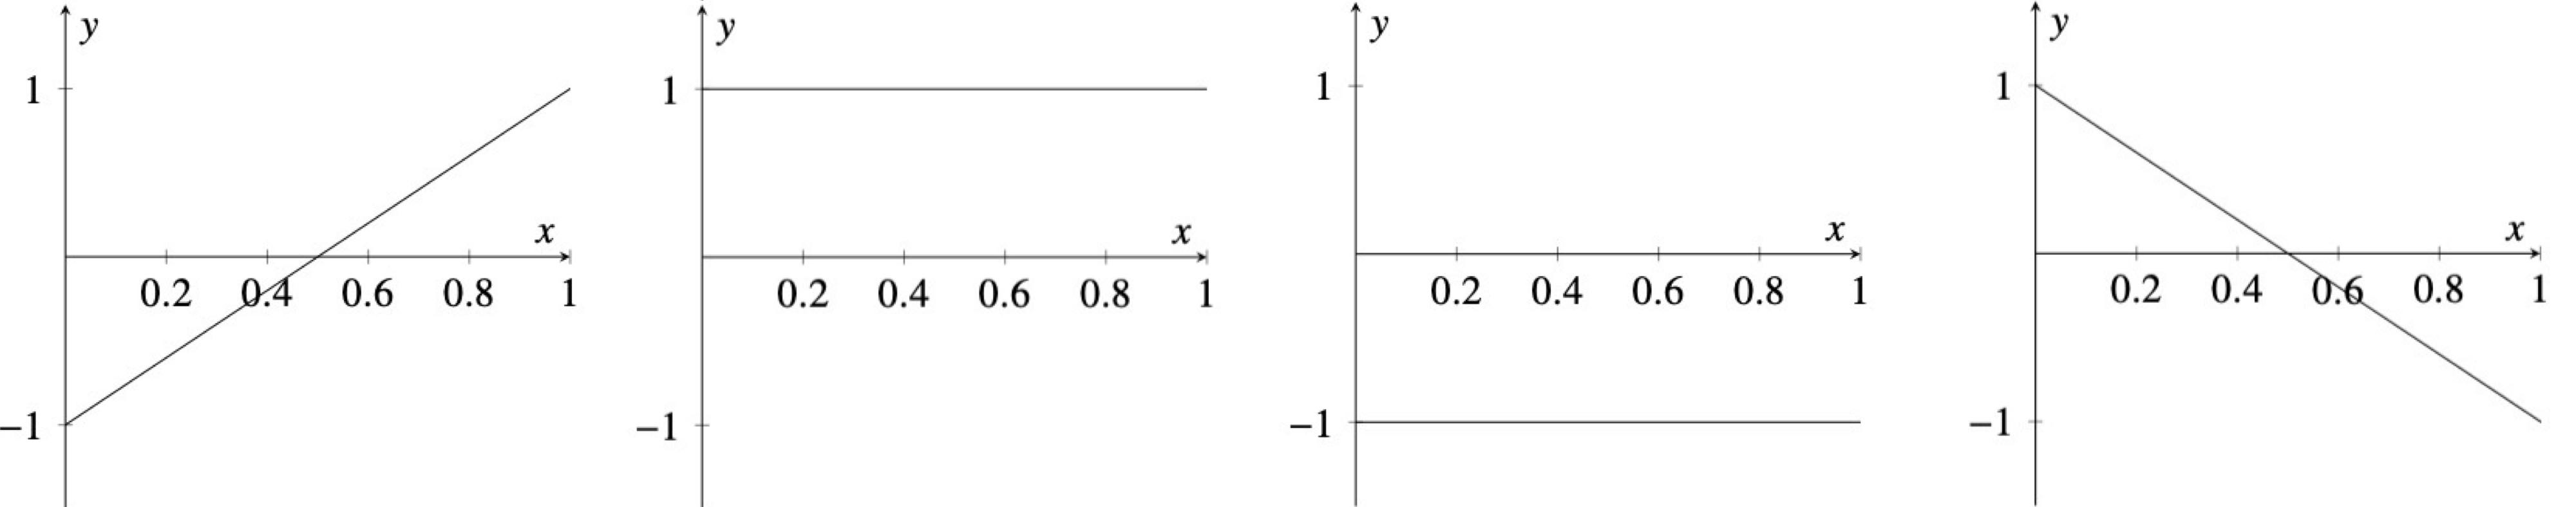
\includegraphics[width=\linewidth]{mainmatter/imgs/states.jpg}
    \caption{visualization of swings, from state1 to state4}
    \label{fig:states}
\end{figure}

Here we display the momentum swings drived from AHP of first three matches.

\begin{figure}[H]
    \centering
    \begin{subfigure}[b]{0.34\textwidth}
        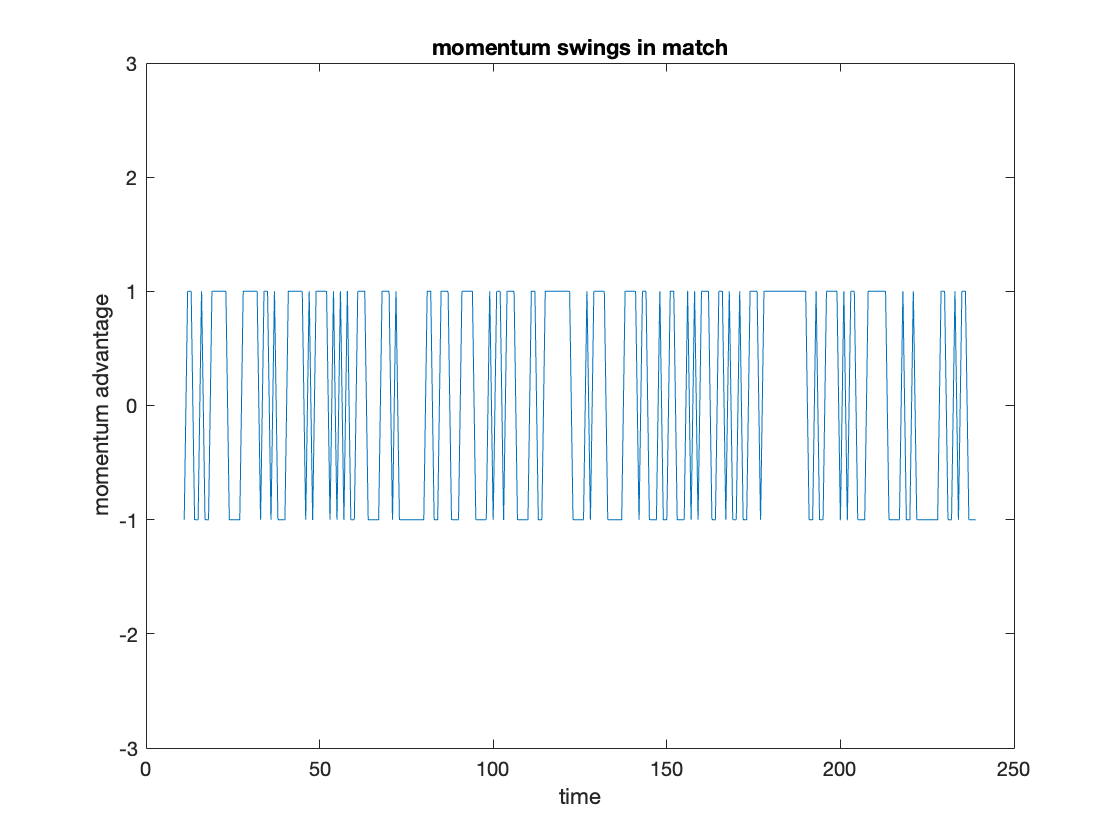
\includegraphics[width=\linewidth]{mainmatter/imgs/swing_match1.png}
        \caption{swings in match 1}
    \end{subfigure}\hspace{-0.02\textwidth}
    \begin{subfigure}[b]{0.34\textwidth}
        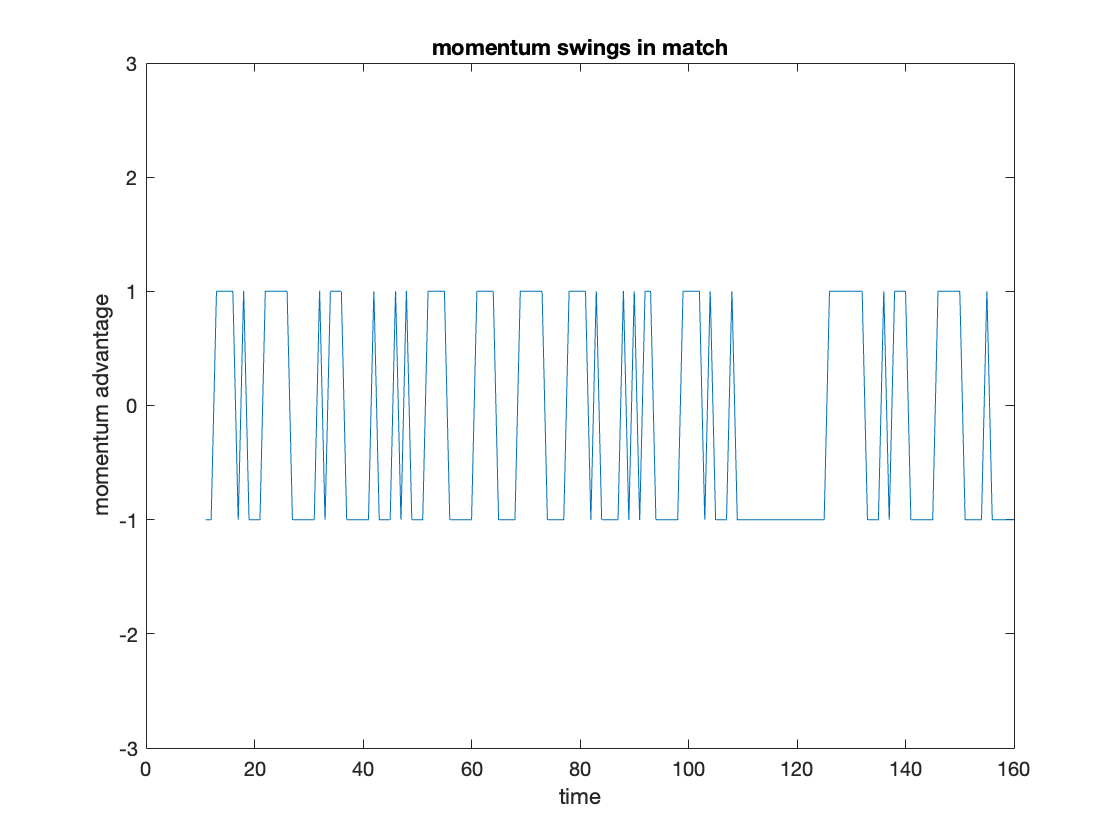
\includegraphics[width=\linewidth]{mainmatter/imgs/swing_match2.png}
        \caption{swings in match 2}
    \end{subfigure}\hspace{-0.02\textwidth}
    \begin{subfigure}[b]{0.34\textwidth}
        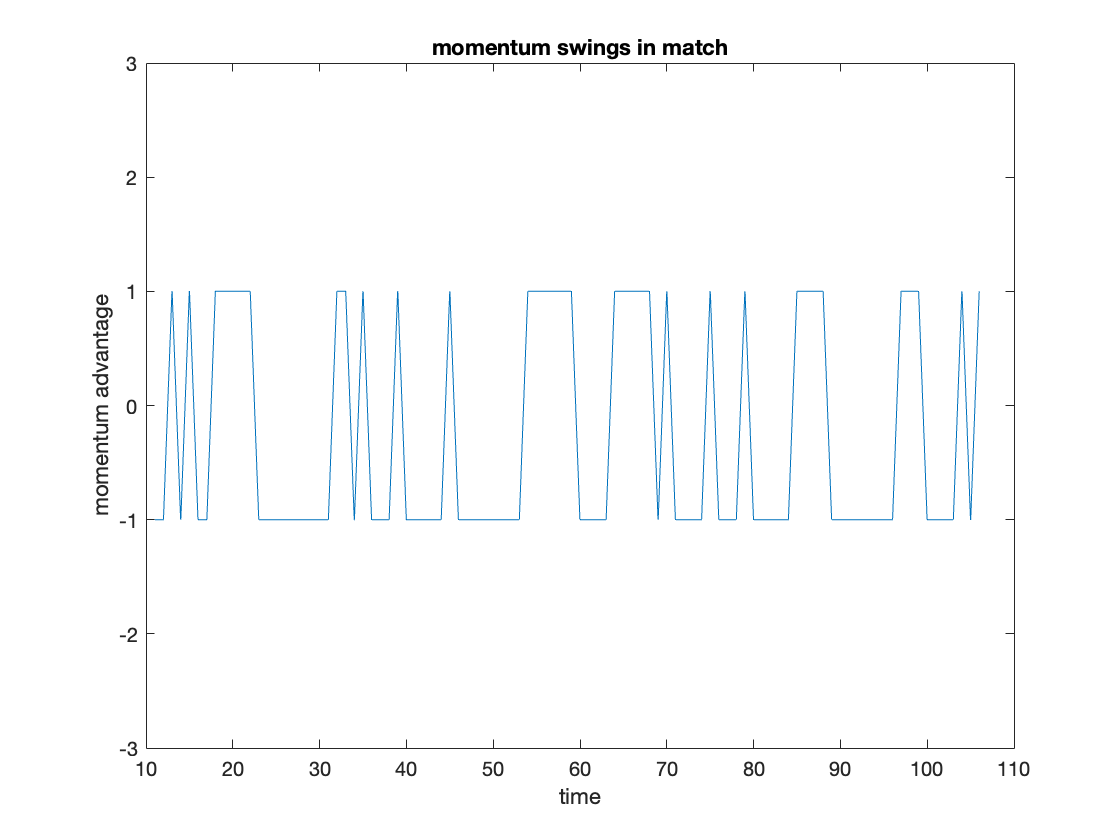
\includegraphics[width=\linewidth]{mainmatter/imgs/swing_match3.png}
        \caption{swings in match 3}
    \end{subfigure}
    \caption{swings in first three matches}
    \label{fig:swings in matches}
\end{figure}


\subsubsection{Data and Label used to train GRU}~{}

To verify all potential factors, meanwhile avoid excessive calculation due to large number of features, we keep track of the following features in each point:

\begin{itemize}
    \item \verb|ace|: represents whether the player hit an ace in the point. This feature is a straightforward rendering of the player's serving ability.
    \item \verb|double_fault|: represents whether the player committed a double fault in the point. By taking this factor into account, we can find out whether the player is stable at serving currently.
    \item \verb|first_serve|: represents whether the player hit the goal in his first serve in the point. This is also a factor reflecting the serving stability of the player.
    \item \verb|fast_win|: represents whether the player won the point after at most 3 rallies. This reflects the player's ability to gain advantage after his serve/return.
    \item \verb|return_depth|: represents the return depth of the player in the point. This factor is key to breaking the opponent's serve. (Who can break a serve if he can't properly return the opponent's serve?)
    \item \verb|winner|: represents whether the player scored by hitting a winner in the point. This shows the player's power at baseline, both forehand and backhand winners are counted.
    \item \verb|net_pt_won|: whether the player scored by coming to the net, reflecting the capability of the player while at net.
    \item \verb|distance|: the running distance of the player in the point. This is an important indicator of the player's energy and stamina.
    \item \verb|unf_err|: whether the player committed an unforced error in the point. Also a indicator of the player's stamina.
    \item \verb|rally|: the rally count in the point. Represents the player's baseline hitting stability as well as his fitness.
    \item \verb|scored_last_point|: whether the player scored the last point or not.
    \item \verb|score_diff|: score difference in the current game. Along with last factor, these factors depict the current situation of the match.
    \item \verb|break_point_diff|: represents the current breakpoint conversion rate of the player. This feature can reflect the player's performance on clutch points.
    \item \verb|speed|: represents the player's serve speed in the point. Yet another feature to show the player's serving ability.
    \item \verb|game_victor|: whether the player won a game in this point.
    \item \verb|set_victor|: whether the player won a set in this point. Along with \verb|game_victor|, these feature also represents the players performance on clutch points.
\end{itemize}

What's more, we want to find out can swings merely be predicted by the technical data,
so that we can give advice to players on skills,
therefore we delete \verb|scored_last_point|, \verb|score_diff|, \verb|game_victor|, \verb|set_victor| before we train a second model.

The label we use is the state of the swing derived from model of AHP.

we use different sets of data to train and derive different models.

\begin{itemize}
    \item First, we will train the model with data from all matches available.
    \item Then, we will train a new model with data from a single player.
    \item Finally, we will train the model with part of available match statistics
\end{itemize}

From the first model, we can find the important factors that affect all players' momentum swings.
From the second model, we can find the important factors that affect 
especially well on that player's momentum swings.
From the third model, we can examine
the generalization ability to accurately predict the swings in irrelevant players and matches.

\subsubsection{Utilizing the Gated Recurrent Unit (GRU) Network}~{}

Gated Recurrent Units (GRUs) are a type of recurrent neural network (RNN) 
architecture that has gained popularity for sequential data processing. 
And it is appropriate for our many(10)-to-many(5) prediction model.

We will focus on a single unit of recurrent neural network to interpret the hidden mathematical principles:
\begin{figure}[H]
    \centering
    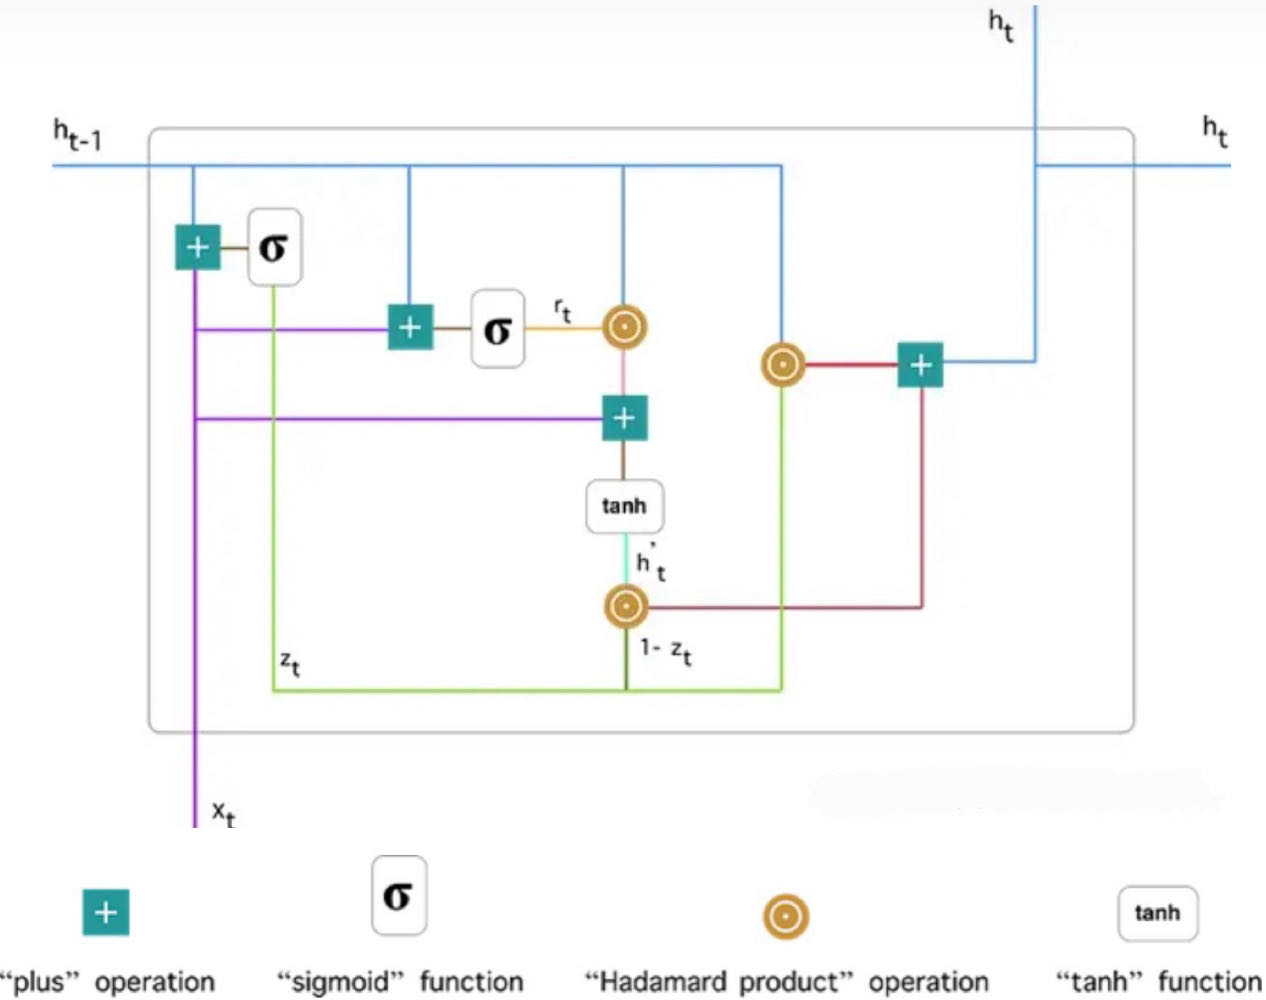
\includegraphics[scale=0.15]{mainmatter/imgs/6.jpg}
    \caption{Structure of GRU}
\end{figure}

\begin{enumerate}
    \item 
    The update gate at time step $t$ is computed using the following formula:  
    $$  z_t = \sigma(W_z \cdot x_t + U_z \cdot h_{t-1})  $$  
    Here, when $x_t$ is input to the network unit, 
    it is multiplied by its own weight $W_z$. 
    Similarly, $h_{t-1}$, which holds the information from the previous $t-1$ units, 
    is multiplied by its own weight $U_z$. These two results are then summed together 
    and passed through a sigmoid activation function to compress the result between 0 and 1. 
  
    \item 
    The essence of the reset gate is for the model to decide how much past information to forget. To compute it, we use:  
    $$  r_t = \sigma(W_r \cdot x_t + U_r \cdot h_{t-1})  $$  

    \item 
    The computation of the new memory content using the reset gate is as follows:  
    $$ h_t'= tanh(Wx_t+r_t\odot Uh_{t-1})$$

    \item 
    The computation for the new memory content $h_t$ using the update gate is as follows:  
    $$ h_t=z_t\odot h_{t-1}+(1-z_t)\odot h_t'$$ 
\end{enumerate}

So, we can predict the momentum swings from the technical data of the past 10 points.

\subsection{Visualization and Analysis}~{}

Out of simplicity, the model shown in this section is trained merely on technical data.

First, we display the model trained on all matches available to 
predict the swings of the play on test data.
To avoid dazzling figure, we minus the swing from AHP with prediction, showing the difference.

Here's the difference of first three matches on training data.

\begin{figure}[H]
    \centering
    \begin{subfigure}[b]{0.34\textwidth}
        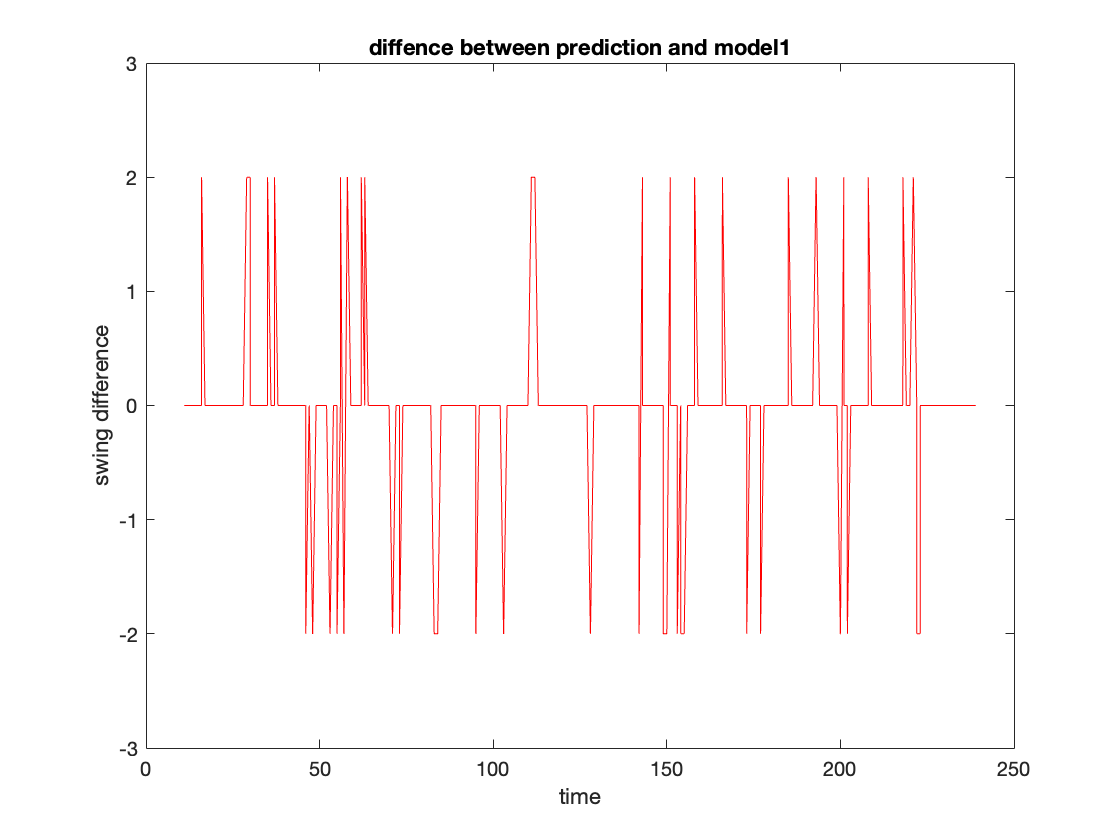
\includegraphics[width=\linewidth]{mainmatter/imgs/swing_diff_match1_overfit.png}
        \caption{difference in match 1}
    \end{subfigure}\hspace{-0.02\textwidth}
    \begin{subfigure}[b]{0.34\textwidth}
        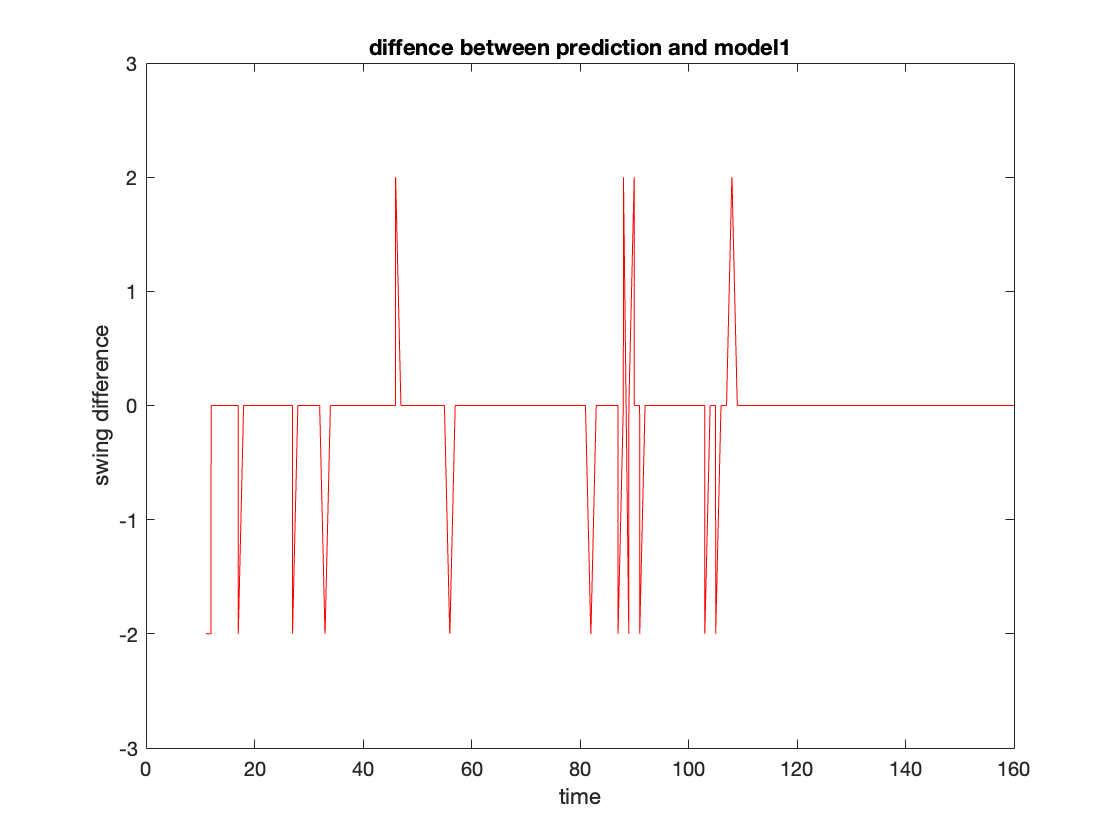
\includegraphics[width=\linewidth]{mainmatter/imgs/swing_diff_match2_overfit.png}
        \caption{difference in match 2}
    \end{subfigure}\hspace{-0.02\textwidth}
    \begin{subfigure}[b]{0.34\textwidth}
        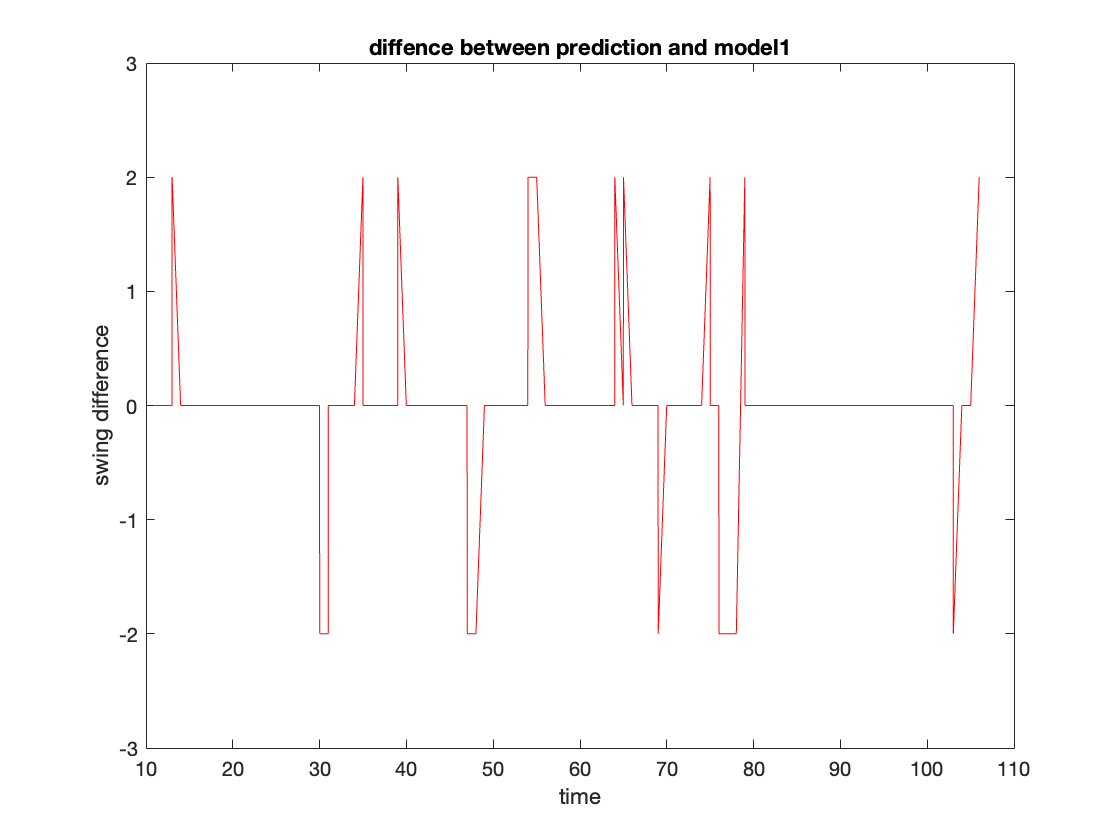
\includegraphics[width=\linewidth]{mainmatter/imgs/swing_diff_match3_overfit.png}
        \caption{difference in match 3}
    \end{subfigure}
    \caption{difference between prediction and AHP model}
    \label{fig:diff swing}
\end{figure}

Here's the difference of first three matches on test data.



Together with other predictions the figures can be concluded as the table below:

\subsubsection{Prediction Error compared with AHP model outcome}

Overlap rate of the prediction model and the result from AHP is?

\paragraph{Factors we may fail to consider}~{}

First of all, the AHP model is not considering all possible factors to momentum.
For example, the.
So the overlap rate's effectiveness is limited.

Then, from the conclusion of problem 2, momentum only has one order of autocorrelation.
So when we try to predict the far future momentum, there's no reason to be accurate.

\subsection{Weight of Factors}~{}

If we can derive the derivative of output with respect to input, we can get the weight of factors.
Although it's difficult to directly acquire derivative, we can use Permutation Feature Importance theory
to avoid getting the derivative.

\subsubsection{Permutation Feature Importance theory}~{}

Permutation Feature Importance theory is used to measure the importance of a feature by calculating 
the increase in the model's prediction error after permuting the feature. A feature is “important” if shuffling its values increases the model error, 
because in this case the model relied on the feature for the prediction. A feature is “unimportant” if 
shuffling its values leaves the model error unchanged, because in this case the model ignored the feature 
for the prediction. 

\begin{algorithm}[H]
    \caption{Permutation Feature Importance}  
    \textbf{Input:} Trained model $\hat{f}$, feature matrix $X$, target vector $y$, error measure $L(y, \hat{f})$.  
      
    Estimate the original model error $e_{orig} = L(y, \hat{f}(X))$ (e.g. mean squared error)  
      
    \textbf{For} each feature $j \in \{1, ..., p\}$ \textbf{do:}  
      
    \quad\quad $\circ$ Generate feature matrix $X_{perm}$ by permuting feature $j$ in the data $X$. This breaks the association between feature $j$ and true outcome $y$.  
      
    \quad\quad $\circ$ Estimate error $e_{perm} = L(Y, \hat{f}(X_{perm}))$ based on the predictions of the permuted data.  
      
    \quad\quad $\circ$ Calculate permutation feature importance as quotient $FI_j = e_{perm} / e_{orig}$ or difference $FI_j = e_{perm} - e_{orig}$  
      
    Sort features by descending FI.
\end{algorithm}

Using the model trained on all matches available, and the above argorithm,
we sort FI and normalize them, then we plot the figure:

\begin{figure}[H]
    \centering
    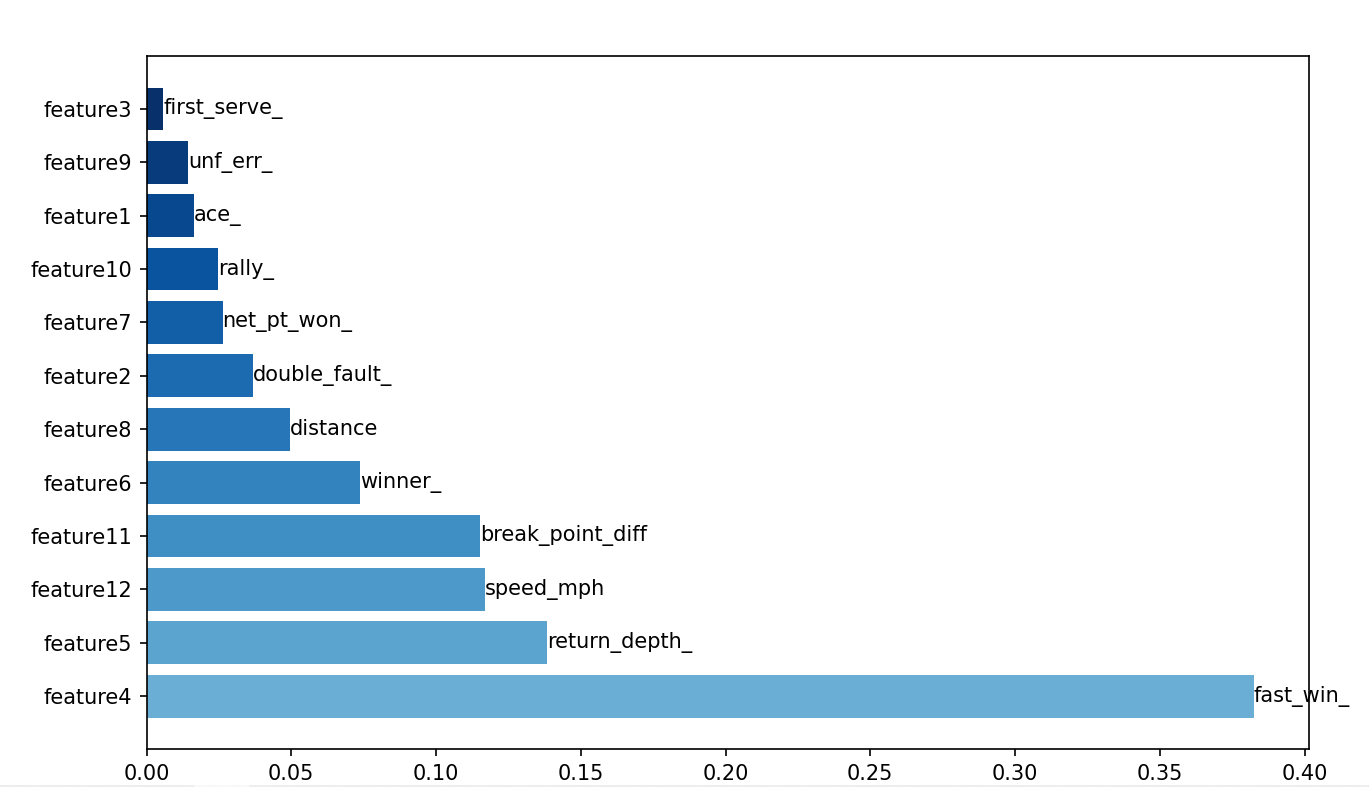
\includegraphics[scale=0.6]{mainmatter/imgs/8.png}
    \caption{feature importance}
\end{figure}

We can see that the most important feature is fast win (rally count $<$ 3 and wins the point),
and the second most important feature is unforced error. Compared to problem 1 (main skill features are
running distance, unforced error and fast win), they coincide. The running distance become insignificant, 
we think it is because this factor is also related to fast win.

The two factors are the most important factors that affect all players.

Using the model with recent score data, we plot the figure:

\begin{figure}[H]
    \centering
    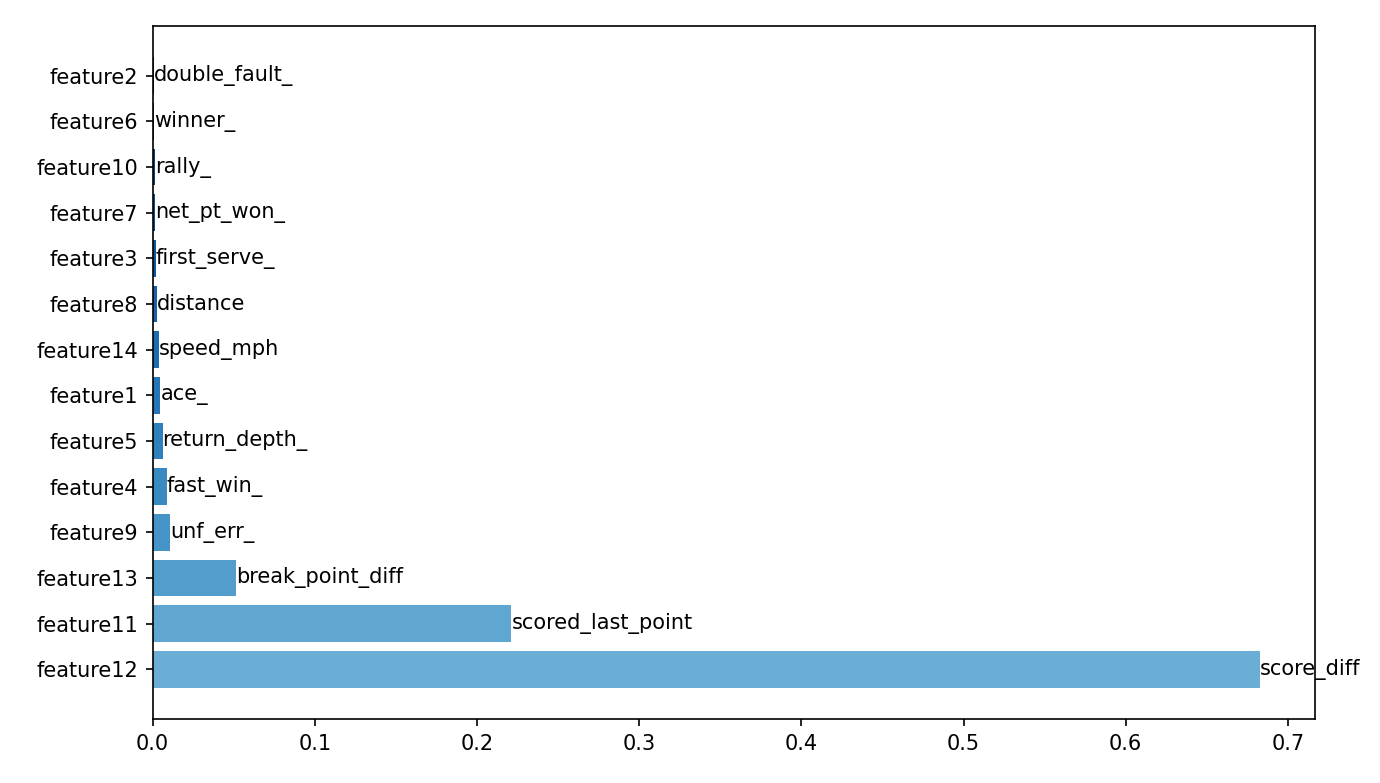
\includegraphics[scale=0.6]{mainmatter/imgs/weight_with_score.jpg}
    \caption{feature importance}
\end{figure}

We can find out that the most important feature is the score difference,
way more important than technical features. 
This is because we find out that the recent score condition is the most direct factor to the momentum.
Now we have expanded our knowledge to problem 2, that among multiple factors
that affect future momentum, 
the recent score condition is the most important.

\subsection{Advice against Opponent Based on Weight of Factors}~{}

As said previously, model trained from match data of a single player,
the factor with bigger weight is extremely effective to this player.

And to give specific advice against the opponent, we choose the model trained on technical data.

We choose three players:rublev(three matches), sinner(four matches), alcaraz(five matches), and 
we use the feature analysis method in problem 3 to find their features, the result is as follows:
\begin{figure}[H]
    \centering
    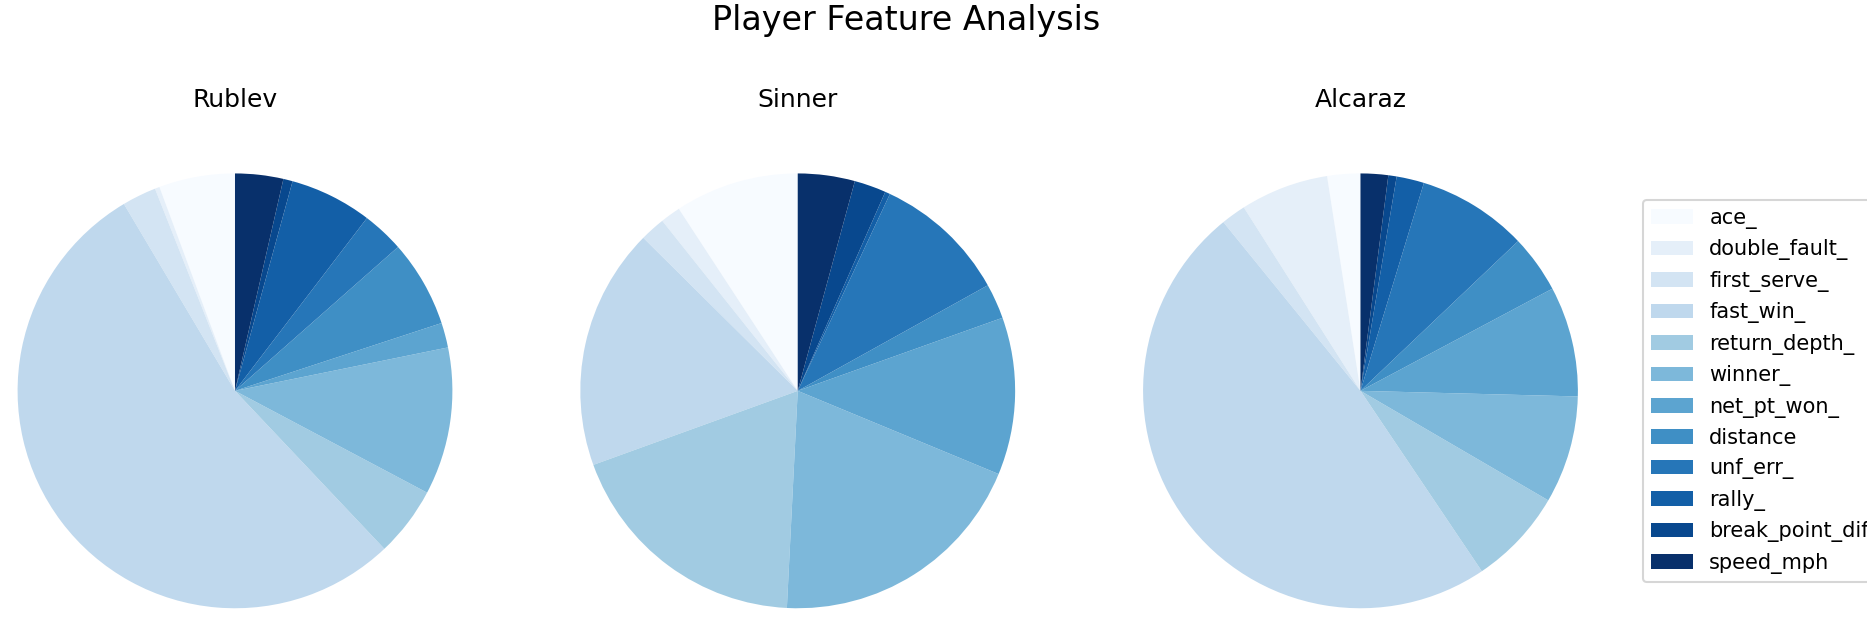
\includegraphics[scale=0.4]{mainmatter/imgs/9.png}
    \caption{features of three players}
\end{figure}
\begin{enumerate}
    \item In comparison to general features, both Rublev and Alcaraz phave significant feature fast win. 
    Therefore, when competing against other players, we recommend them to emphasize the rhythm of seizing 
    the early shots. For example, they can focus more on the quality of their serves, 
    progressively achieving a fast win to enhance their momentum. 
    \item Additionally, Rublev is hardly affected by negative factors such as double fault and 
    unforced error. Hence, in matches, there is no need for him to worry about occasional mistakes; 
    instead, he can play boldly.
    \item For Sinner, his technical characteristics are markedly different. 
    Important features for him are winners and return depth. Consequently, 
    we advise Sinner to fully exploit his strong scoring abilities of winner points
    and utilize his control over return depth to steer the course of the match and establish an advantage.

\end{enumerate}

Now we have finished Problem 3.